 We conducted two studies using patient data associated with chronic disease.  The first experiment is designed to group hepatitis patients with similar stages of liver decline by modeling the dynamics of patient lab result.  The second uses administrative indicating physicians orders for glucose tests during hospital stays and aims to group patients that are at high and low risk of diabetes associated hospitalizations.


\subsection{Hepatitis Experiments}
%‘Hepatitis’ is a Greek word with the root ‘hepat’ meaning liver and the suffix ‘itis’
%indicating inflammation. It is used to describe a class of viruses that are associated
%with liver inflammation that can become chronic, and progress to more severe stages
%that may result in permanent scaring of liver tissue, a condition known as cirrhosis.
Using the data set described in Section~\ref{data}, and given threshold for low, normal and high observation values for each test, we constructed the model structure.  Based on an initial run using six lab tests that were selected due to known associations with liver decline, three, the PLT, ALB, and ZZT tests, resulted in good cluster assignments, with PLT performing the best  based on the b-cubed metric~\cite{Bagga}, which is the harmonic mean of the average pointwise precision and recall for the data set.  B-cubed is the only well-established metric that satisfies the full set of formal constraints proposed by researchers and validated by human assessors~\cite{Amigo}.

\subsubsection{Extrinsic Validation}
To validate the results of clustering platelet count values for the hepatitis data set, we used grading and staging data from liver biopsies a gold standard.  Also, we compare our results of a previous method that used a feature extraction approach~\cite{Hirano07} and selected only those patients with hepatitis C and no indication of interferon therapy.  The results of semiparametric clustering (SP-B) are reported for 94 of these patients based on clustering PLT (platelet) and ALB (albumin) lab tests, and for PLT only.

Figure~\ref{hepC} shows average pointwise precision on the x-axis, recall on the y-axis and the B-cubed value  as a gradient value.  Detailed scores appear in Table ~\ref{scBayestable}.

\begin{figure}[t]
\vskip 0.2in
\begin{center}
\centerline{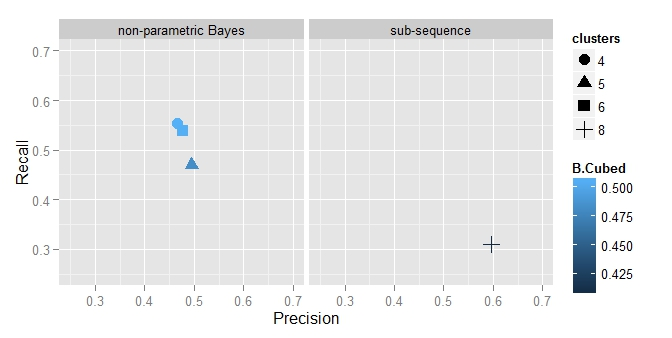
\includegraphics[width=\columnwidth]{fig/hepC.jpeg}}
\caption{Comparison of semiparametric clustering with a reported benchmark}
\label{hepC}
\end{center}
\vskip -0.2in
\end{figure}

\begin{table}[ht]
\caption{Validation scores for spectral (SC) and nonparametric Bayes (Bayes) clustering on all hepatitis patients.}
\label{scBayestable}
\vskip 0.15in
\begin{center}
\begin{small}
\begin{sc}
\begin{tabular}{lcccr}
\hline
\abovespace\belowspace
method	& k	& P	& R	& B-Cubed \\
\hline
\abovespace
sub-sequence	& 8& 0.60& 0.31& 0.41 \\
SP-B(PLT)		& 5& 0.49& 0.42& 0.45 \\
\textbf{SP-B}	        & \textbf{4}& \textbf{0.47}& \textbf{0.55}& \textbf{0.51 }\\
SP-B	        & 5& 0.50& 0.47& 0.48 \\

\belowspace
\textbf{SP-B}	        &\textbf{ 6}& \textbf{0.48}& \textbf{0.54}& \textbf{0.51} \\
\hline
\end{tabular}
\end{sc}
\end{small}
\end{center}
\vskip -0.1in
\end{table}

Also, we apply our method to the entire data set, including those on interferon therapy and patients with hepatitis B, and compare it with an alternative nonparametric method, spectral clustering.  The results appear in Figure~\ref{allHep} and are detailed in Table~\ref{allHepTable}.

\begin{figure}[t]
\vskip 0.2in
\begin{center}
\centerline{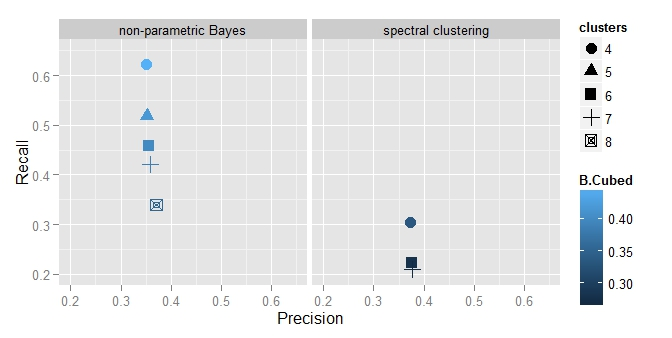
\includegraphics[width=\columnwidth]{fig/allHep.jpeg}}
\caption{B-cubed value for different methods and $k$ values for the hepatitis data set}
\label{allHep}
\end{center}
\vskip -0.2in
\end{figure}


\begin{table}[ht]
\caption{B-cubed value for spectral (SP-SC) and nonparametric Bayes (SP-B) clustering, all hepatitis patients.}
\label{allHepTable}
\vskip 0.15in
\begin{center}
\begin{small}
\begin{sc}
\begin{tabular}{lcccr}
\hline
\abovespace\belowspace
method	& k	& P	& R	& B-Cubed \\
\hline
\abovespace
SP-SC	         & 6	& 0.38& 0.22& 0.28\\
SP-SC	         & 7	& 0.38& 0.21& 0.27\\
\textbf{SP-B }       & \textbf{4}	& \textbf{0.35}& \textbf{0.62}& \textbf{0.45}\\
SP-B	     & 5	& 0.35& 0.52& 0.42\\
SP-B	     & 6	& 0.36& 0.46& 0.40\\
\belowspace
SP-B	     & 7	& 0.36& 0.42& 0.39\\
\hline
\end{tabular}
\end{sc}
\end{small}
\end{center}
\vskip -0.1in
\end{table}


\subsection{Diabetes Experiments}
The glucose testing data was processed before state estimation.  Creating a new vector, we set the observation value to the number of days contiguous tests were ordered.  For example, and measurement sequence of $[1,0,0,0,1,1,1,1]$ would consist of two observations, 1 and 4.  We estimated $n$, the number of states for the models using a non-parametric Bayesian density estimator.  Since the number of states and the continuous nature of the model should not be too large, the upper-bound on the number for density estimation was set to a maximum of five.


\subsubsection{Intrinsic Validation}
When a gold standard is unavailable to evaluate clustering performance, heuristics can be used to assess the intrinsic quality of clusters.  For each point in the data set, the silhouette method is defined by the different of average dissimilarity of a point to members or its own cluster with that of the `neighboring' cluster over the max of these two dissimilarity measures.

Based on the results of applying our clustering approach to the glucose testing data, Figure~\ref{sil} shows the silhouette for the assignments and Table~\ref{stats} shows cluster averages including: number of members, total glucose tests, number of hospital admissions, entropy of the measurement sequence, and fraction of days measured.

\begin{figure}[t]
\begin{center}
\centerline{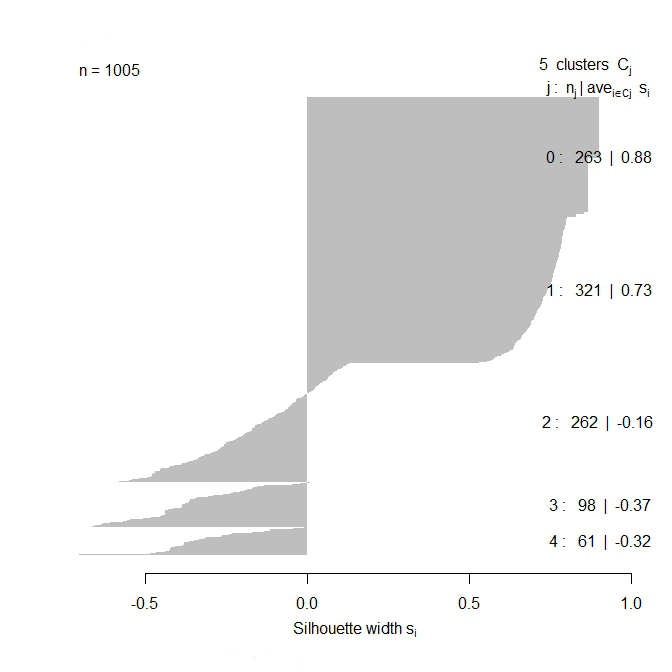
\includegraphics[width=\columnwidth]{fig/sil.jpeg}}
\caption{Silhouettes by cluster for 4-state model.}
\label{sil}
\end{center}
\vskip -0.2in
\end{figure}


\begin{table}[ht]
\caption{Time series statistics aggregated by cluster}
\label{stats}
\vskip 0.15in
\begin{center}
\begin{small}
\begin{sc}
\begin{tabular}{lccccr}
\hline
\abovespace\belowspace
k 	&n 	&Tests 	&Stays 	&Entropy 	&Fraction \\
\hline
\abovespace
0	&263	&8.6	&7.81	&0.05	&0.01\\
1	&321	&39.64	&16.98	&0.14	&0.04\\
2	&262	&22.00	     &13.53	&0.10	&0.02\\
3	&98	    &24.77	&11.38	&0.10	&0.02\\
4	&61	    &16.74	&7.69	&0.08	&0.02\\
\belowspace
T 	&1005	&24.08	&12.57	&0.10	&0.02\\
\hline
\end{tabular}
\end{sc}
\end{small}
\end{center}
\vskip -0.1in
\end{table}



